% GNUPLOT: LaTeX picture with Postscript
\begingroup
  \makeatletter
  \providecommand\color[2][]{%
    \GenericError{(gnuplot) \space\space\space\@spaces}{%
      Package color not loaded in conjunction with
      terminal option `colourtext'%
    }{See the gnuplot documentation for explanation.%
    }{Either use 'blacktext' in gnuplot or load the package
      color.sty in LaTeX.}%
    \renewcommand\color[2][]{}%
  }%
  \providecommand\includegraphics[2][]{%
    \GenericError{(gnuplot) \space\space\space\@spaces}{%
      Package graphicx or graphics not loaded%
    }{See the gnuplot documentation for explanation.%
    }{The gnuplot epslatex terminal needs graphicx.sty or graphics.sty.}%
    \renewcommand\includegraphics[2][]{}%
  }%
  \providecommand\rotatebox[2]{#2}%
  \@ifundefined{ifGPcolor}{%
    \newif\ifGPcolor
    \GPcolortrue
  }{}%
  \@ifundefined{ifGPblacktext}{%
    \newif\ifGPblacktext
    \GPblacktextfalse
  }{}%
  % define a \g@addto@macro without @ in the name:
  \let\gplgaddtomacro\g@addto@macro
  % define empty templates for all commands taking text:
  \gdef\gplbacktext{}%
  \gdef\gplfronttext{}%
  \makeatother
  \ifGPblacktext
    % no textcolor at all
    \def\colorrgb#1{}%
    \def\colorgray#1{}%
  \else
    % gray or color?
    \ifGPcolor
      \def\colorrgb#1{\color[rgb]{#1}}%
      \def\colorgray#1{\color[gray]{#1}}%
      \expandafter\def\csname LTw\endcsname{\color{white}}%
      \expandafter\def\csname LTb\endcsname{\color{black}}%
      \expandafter\def\csname LTa\endcsname{\color{black}}%
      \expandafter\def\csname LT0\endcsname{\color[rgb]{1,0,0}}%
      \expandafter\def\csname LT1\endcsname{\color[rgb]{0,1,0}}%
      \expandafter\def\csname LT2\endcsname{\color[rgb]{0,0,1}}%
      \expandafter\def\csname LT3\endcsname{\color[rgb]{1,0,1}}%
      \expandafter\def\csname LT4\endcsname{\color[rgb]{0,1,1}}%
      \expandafter\def\csname LT5\endcsname{\color[rgb]{1,1,0}}%
      \expandafter\def\csname LT6\endcsname{\color[rgb]{0,0,0}}%
      \expandafter\def\csname LT7\endcsname{\color[rgb]{1,0.3,0}}%
      \expandafter\def\csname LT8\endcsname{\color[rgb]{0.5,0.5,0.5}}%
    \else
      % gray
      \def\colorrgb#1{\color{black}}%
      \def\colorgray#1{\color[gray]{#1}}%
      \expandafter\def\csname LTw\endcsname{\color{white}}%
      \expandafter\def\csname LTb\endcsname{\color{black}}%
      \expandafter\def\csname LTa\endcsname{\color{black}}%
      \expandafter\def\csname LT0\endcsname{\color{black}}%
      \expandafter\def\csname LT1\endcsname{\color{black}}%
      \expandafter\def\csname LT2\endcsname{\color{black}}%
      \expandafter\def\csname LT3\endcsname{\color{black}}%
      \expandafter\def\csname LT4\endcsname{\color{black}}%
      \expandafter\def\csname LT5\endcsname{\color{black}}%
      \expandafter\def\csname LT6\endcsname{\color{black}}%
      \expandafter\def\csname LT7\endcsname{\color{black}}%
      \expandafter\def\csname LT8\endcsname{\color{black}}%
    \fi
  \fi
    \setlength{\unitlength}{0.0500bp}%
    \ifx\gptboxheight\undefined%
      \newlength{\gptboxheight}%
      \newlength{\gptboxwidth}%
      \newsavebox{\gptboxtext}%
    \fi%
    \setlength{\fboxrule}{0.5pt}%
    \setlength{\fboxsep}{1pt}%
\begin{picture}(7370.00,2494.00)%
    \gplgaddtomacro\gplbacktext{%
      \csname LTb\endcsname%%
      \put(644,616){\makebox(0,0)[r]{\strut{}0}}%
      \put(644,899){\makebox(0,0)[r]{\strut{}0.2}}%
      \put(644,1182){\makebox(0,0)[r]{\strut{}0.4}}%
      \put(644,1465){\makebox(0,0)[r]{\strut{}0.6}}%
      \put(644,1748){\makebox(0,0)[r]{\strut{}0.8}}%
      \put(644,2031){\makebox(0,0)[r]{\strut{}1}}%
      \put(1006,462){\makebox(0,0){\strut{}$16$}}%
      \put(1448,462){\makebox(0,0){\strut{}$32$}}%
      \put(1891,462){\makebox(0,0){\strut{}$64$}}%
      \put(2334,462){\makebox(0,0){\strut{}$128$}}%
      \put(2776,462){\makebox(0,0){\strut{}$256$}}%
      \put(3219,462){\makebox(0,0){\strut{}$512$}}%
      \put(3661,462){\makebox(0,0){\strut{}$1024$}}%
    }%
    \gplgaddtomacro\gplfronttext{%
      \csname LTb\endcsname%%
      \put(129,1323){\makebox(0,0){\strut{}$\rho$}}%
      \put(2321,154){\makebox(0,0){\strut{}$n$}}%
      \put(2321,2163){\makebox(0,0){\strut{}Single-phase Poisson problem}}%
    }%
    \gplgaddtomacro\gplbacktext{%
      \csname LTb\endcsname%%
      \put(4034,616){\makebox(0,0)[r]{\strut{}}}%
      \put(4034,899){\makebox(0,0)[r]{\strut{}}}%
      \put(4034,1182){\makebox(0,0)[r]{\strut{}}}%
      \put(4034,1465){\makebox(0,0)[r]{\strut{}}}%
      \put(4034,1748){\makebox(0,0)[r]{\strut{}}}%
      \put(4034,2031){\makebox(0,0)[r]{\strut{}}}%
      \put(4538,462){\makebox(0,0){\strut{}$64$}}%
      \put(5144,462){\makebox(0,0){\strut{}$128$}}%
      \put(5750,462){\makebox(0,0){\strut{}$256$}}%
      \put(6355,462){\makebox(0,0){\strut{}$512$}}%
      \put(6961,462){\makebox(0,0){\strut{}$1024$}}%
    }%
    \gplgaddtomacro\gplfronttext{%
      \csname LTb\endcsname%%
      \put(5711,154){\makebox(0,0){\strut{}$n$}}%
      \put(5711,2163){\makebox(0,0){\strut{}Multi-phase elliptic interface problem}}%
    }%
    \gplbacktext
    \put(0,0){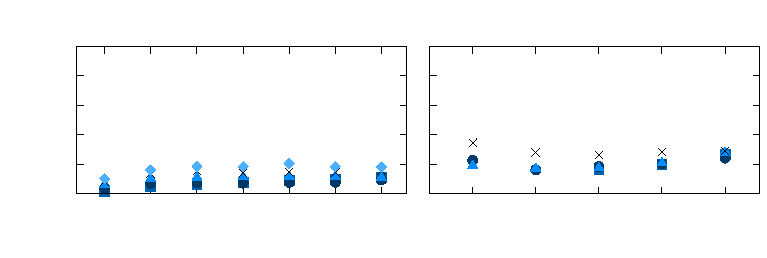
\includegraphics{implicit-results}}%
    \gplfronttext
  \end{picture}%
\endgroup
